\subsubsection{Graph Format}

The control flow graph is a directed graph that is generally not acyclic because of cycles created by loop structures. Its nodes represent states of the program, whereas its edges represent transitions between those states. Edges can be annotated with statements or expressions that change the state of the program. Here is an example of a very simple control flow graph:

\begin{figure}[h]
  \centering
  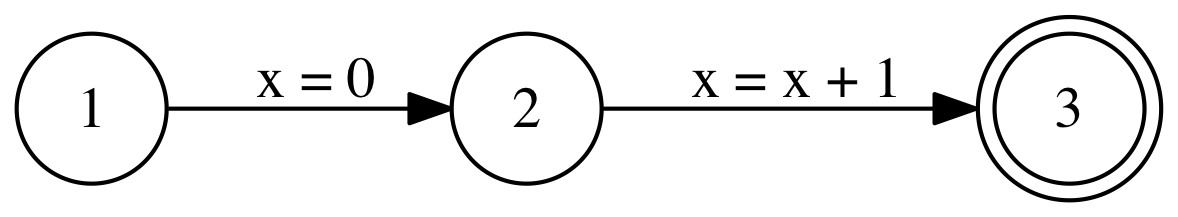
\includegraphics[width=0.7\textwidth]{sections/algorithm/images/simple-cfg}
\end{figure}

It represents the following simple JavaScript program:

\begin{minted}[linenos,xleftmargin=0.6cm]{js}
var x = 0;
x = x + 1;
\end{minted}

The abstract syntax tree in ESTree format looks like this:

\begin{minted}[linenos,baselinestretch=0.93,xleftmargin=0.75cm]{json}
{
  "type": "Program",
  "body": [
    {
      "type": "VariableDeclaration",
      "declarations": [
        {
          "type": "VariableDeclarator",
          "id": {
            "type": "Identifier",
            "name": "x"
          },
          "init": {
            "type": "Literal",
            "value": 0
          }
        }
      ],
      "kind": "var"
    },
    {
      "type": "ExpressionStatement",
      "expression": {
        "type": "AssignmentExpression",
        "operator": "=",
        "left": {
          "type": "Identifier",
          "name": "x"
        },
        "right": {
          "type": "BinaryExpression",
          "operator": "+",
          "left": {
            "type": "Identifier",
            "name": "x"
          },
          "right": {
            "type": "Literal",
            "value": 1
          }
        }
      }
    }
  ]
}
\end{minted}
